\whiteBGstarBegin
\setcounter{section}{0}
\section{Trắc nghiệm}
\begin{enumerate}[label=\bfseries Câu \arabic*:]
	
	
	\item \mkstar{1}
	
	\cauhoi
	{Trong một mạch kín gồm nguồn điện có suất điện động $\calE$, điện trở trong $r$ và mạch ngoài có điện trở $R$. Hệ thức nêu lên mỗi quan hệ giữa các đại lượng trên với cường độ dòng điện $I$ chạy trong mạch là
		\begin{mcq}(4)
			\item $I=\dfrac{\calE}{R}$.
			\item $I=\calE \sqrt{\dfrac{\calE}{R}}$.
			\item $I=\dfrac{\calE}{R+r}$.
			\item $I=\dfrac{\calE}{r}$.
		\end{mcq}
		
	}
	\loigiai
	{	\textbf{Đáp án: C.}
		
		Định luật Ôm đối với toàn mạch: Cường độ dòng điện chạy trong mạch điện kín tỉ lệ thuận với suất điện động cua nguồn điện và tỉ lệ nghịch với điện trở toàn phần của mạch đó:
		$$I=\dfrac{\calE}{R+r},$$
		với $R$ là điện trở mạch ngoài; $r$ là điện trở trong của nguồn điện.
	}
	\item \mkstar{1}
	
	\cauhoi
	{Trong mạch điện kín gồm nguồn điện có suất điện động $\calE$, điện trở trong $r$ và mạch ngoài có điện trở $R$. Khi có hiện tượng đoản mạch thì cường độ dòng điện trong mạch $I$ được xác định bằng công thức:
		\begin{mcq}(4)
			\item $I=\dfrac{\calE}{r}$.
			\item $I=\calE r$.
			\item $I=\dfrac{r}{\calE}$.
			\item $I=\dfrac{\calE}{R+r}$.
		\end{mcq}
		
	}
	\loigiai
	{	\textbf{Đáp án: A.}
		
		Định luật Ôm đối với toàn mạch:
		$$I=\dfrac{\calE}{R+r}.$$
		
		Khi có hiện tượng đoản mạch ($R=0$) thì cường độ dòng điện trong mạch là
		$$I=\dfrac{\calE}{r}.$$
	}
	\item \mkstar{2}
	
	\cauhoi
	{Một điện trở $\SI{4}{\Omega}$ được mắc vào nguồn điện có suất điện động $\calE = \SI{1.5}{V}$ để tạo thành một mạch điện kín thì công suất tỏa nhiệt trên điện trở này bằng $\SI{0.36}{W}$. Hiệu điện thế giữa hai đầu điện trở $R$ là
		\begin{mcq}(4)
			\item 1 V.
			\item $\SI{1.2}{V}$.
			\item $\SI{1.4}{V}$.
			\item $\SI{1.6}{V}$.
		\end{mcq}
		
	}
	\loigiai
	{	\textbf{Đáp án: B.}
		
		Hiệu điện thế giữa hai đầu điện trở:
		$$\calP = \dfrac{U^2}{R} \Rightarrow U=\SI{1.2}{V}.$$
	}
	\item \mkstar{2}
	
	\cauhoi
	{Một điện trở $\SI{4}{\Omega}$ được mắc vào nguồn điện có suất điện động $\calE = \SI{1.5}{V}$ để tạo thành một mạch điện kín thì công suất tỏa nhiệt trên điện trở này bằng $\SI{0.36}{W}$. Điện trở trong của nguồn điện là
		\begin{mcq}(4)
			\item $\SI{0.5}{\Omega}$.
			\item $\SI{0.25}{\Omega}$.
			\item $\SI{5}{\Omega}$.
			\item $\SI{1}{\Omega}$.
		\end{mcq}
		
	}
	\loigiai
	{	\textbf{Đáp án: D.}
		
		Hiệu điện thế giữa hai đầu điện trở:
		$$\calP = \dfrac{U^2}{R} \Rightarrow U=\SI{1.2}{V}.$$
		
		Cường độ dòng điện chạy trong mạch:
		$$\calP = UI \Rightarrow I=\SI{0.3}{A}.$$
		
		Áp dụng định luật Ôm toàn mạch:
		$$I=\dfrac{\calE}{R+r} \Rightarrow r = \SI{1}{\Omega}.$$
	}
	\item \mkstar{2}
	
	\cauhoi
	{Hai bóng đèn có điện trở $\SI{5}{\Omega}$ mắc song song với nhau và nối vào một nguồn điện có điện trở trong $\SI{1}{\Omega}$ thì cường độ dòng điện trong mạch là $\xsi{12/7}{A}$. Khi tháo một bóng đèn ra thì cường độ dòng điện trong mạch là
		\begin{mcq}(4)
			\item $\xsi{6/5}{A}$.
			\item 1 A.
			\item $\xsi{5/6}{A}$.
			\item 0 A.
		\end{mcq}
		
	}
	\loigiai
	{	\textbf{Đáp án: B.}
		
		Áp dụng định luật Ôm toàn mạch:
		$$I=\dfrac{\calE}{r + \dfrac{R R}{R + R}} \Rightarrow \calE = \SI{6}{V}.$$
		
		Khi tháo một bóng đèn ra, áp dụng định luật Ôm toàn mạch:
		$$I' = \dfrac{\calE}{r + R} = \SI{1}{A}.$$
	}
	\item \mkstar{2}
	
	\cauhoi
	{Cho đoạn mạch gồm điện trở $R_1=\SI{100}{\Omega}$ mắc nối tiếp với điện trở $R_2=\SI{200}{\Omega}$, hiệu điện thế giữa hai đầu đoạn mạch là $\SI{12}{V}$. Hiệu điện thế giữa hai đầu điện trở $R_1$ là
		\begin{mcq}(4)
			\item $U_1 = \SI{1}{V}$.
			\item $U_1=\SI{8}{V}$.
			\item $U_1=\SI{4}{V}$.
			\item $U_1=\SI{6}{V}$.
		\end{mcq}
		
	}
	\loigiai
	{	\textbf{Đáp án: C.}
		
		Cường độ dòng điện qua mạch:
		$$I=\dfrac{U}{R} = \dfrac{U}{R_1 + R_2} = \SI{0.04}{A}.$$
		
		Hiệu điện thế giữa hai đầu $R_1$:
		$$U_1 = I R_1 = \SI{4}{V}.$$
	}
	\item \mkstar{2}
	
	\cauhoi
	{Cho đoạn mạch gồm điện trở $R_1=\SI{100}{\Omega}$ mắc nối tiếp với điện trở $R_2=\SI{200}{\Omega}$, hiệu điện thế giữa hai đầu đoạn mạch là $\SI{12}{V}$. Hiệu điện thế giữa hai đầu điện trở $R_2$ là
		\begin{mcq}(4)
			\item $U_1=\SI{1}{V}$.
			\item $U_1=\SI{8}{V}$.
			\item $U_1=\SI{4}{V}$.
			\item $U_1=\SI{6}{V}$.
		\end{mcq}
		
	}
	\loigiai
	{	\textbf{Đáp án: B.}
		
		Cường độ dòng điện qua mạch:
		$$I=\dfrac{U}{R} = \dfrac{U}{R_1 + R_2} = \SI{0.04}{A}.$$
		
		Hiệu điện thế giữa hai đầu $R_2$:
		$$U_2 = I R_2= \SI{8}{V}.$$
	}
	\item \mkstar{2}
	
	\cauhoi
	{Một nguồn điện có suất điện động $\calE = \SI{12}{V}$, điện trở trong $\SI{2}{\Omega}$ nối tiếp với điện trở $R$ tạo thành mạch điện kín. Công suất tiêu thụ trên điện trở $R$ bằng 16 W. Biết $R>\SI{2}{\Omega}$, giá trị của $R$ là
		\begin{mcq}(4)
			\item $\SI{3}{\Omega}$.
			\item $\SI{6}{\Omega}$.
			\item $\SI{5}{\Omega}$.
			\item $\SI{4}{\Omega}$.
		\end{mcq}
		
	}
	\loigiai
	{	\textbf{Đáp án: D.}
		
		Công suất tiêu thụ trên điện trở:
		$$\calP = I^2 R \Rightarrow \calP = \left(\dfrac{\calE}{R + r}\right)^2 R \Rightarrow R^2 + 2Rr + r^2 = \dfrac{\calE^2 R}{\calP}.$$
		
		Giải phương trình bậc hai trên, tính được $R=\SI{4}{\Omega}$ hoặc $R=\SI{1}{\Omega}$.
		
		Mà theo đề bài thì $R>\SI{2}{\Omega}$, nên giá trị $R$ là $R=\SI{4}{\Omega}$.
	}
	\item \mkstar{2}
	
	\cauhoi
	{Cho mạch điện gồm nguồn điện ($\calE=\SI{12}{V}$, $r=\SI{1}{\Omega}$) nối với mạch ngoài gồm 3 điện trở mắc nối tiếp: $R_1=\SI{3}{\Omega}$, $R_2=\SI{6}{\Omega}$, $R_3=\SI{5}{\Omega}$. Tính hiệu điện thế giữa hai đầu điện trở $R_2$.
		\begin{mcq}(4)
			\item $\SI{3.5}{V}$.
			\item $\SI{4.8}{V}$.
			\item $\SI{2.5}{V}$.
			\item $\SI{4.5}{V}$.
		\end{mcq}
		
	}
	\loigiai
	{	\textbf{Đáp án: B.}
		
		Cường độ dòng điện qua mạch:
		$$I=\dfrac{\calE}{R + r} = \dfrac{\calE}{R_1 + R_2 + R_3 + r} = \SI{0.8}{A}.$$
		
		Hiệu điện thế giữa hai đầu $R_2$:
		$$U_2 = I R_2 = \SI{4.8}{V}.$$
	}
	\item \mkstar{2}
	
	\cauhoi
	{Cho mạch điện gồm nguồn điện ($\calE=\SI{12}{V}$, $r=\SI{1}{\Omega}$) nối với mạch ngoài gồm 3 điện trở mắc nối tiếp: $R_1=\SI{3}{\Omega}$, $R_2=\SI{6}{\Omega}$, $R_3=\SI{5}{\Omega}$. Tính hiệu điện thế giữa hai đầu đoạn mạch.
		\begin{mcq}(4)
			\item $\SI{6.5}{V}$.
			\item $\SI{11.8}{V}$.
			\item $\SI{11.2}{V}$.
			\item $\SI{6.2}{V}$.
		\end{mcq}
		
	}
	\loigiai
	{	\textbf{Đáp án: C.}
		
		Cường độ dòng điện qua mạch:
		$$I=\dfrac{\calE}{R + r} = \dfrac{\calE}{R_1 + R_2 + R_3 + r} = \SI{0.8}{A}.$$
		
		Hiệu điện thế giữa hai đầu đoạn mạch:
		$$U=IR = \SI{11.2}{V}.$$
	}
	\item \mkstar{2}
	
	\cauhoi
	{Cho mạch điện gồm nguồn điện ($\calE=\SI{12}{V}$, $r=\SI{1}{\Omega}$) nối với mạch ngoài gồm 3 điện trở mắc song song: $R_1=\SI{3}{\Omega}$, $R_2=\SI{6}{\Omega}$, $R_3=\SI{5}{\Omega}$. Tính hiệu điện thế giữa hai đầu điện trở $R_2$.
		\begin{mcq}(4)
			\item $\SI{11.8}{V}$.
			\item $\SI{10.2}{V}$.
			\item $\SI{11.2}{V}$.
			\item $\SI{10.4}{V}$.
		\end{mcq}
		
	}
	\loigiai
	{	\textbf{Đáp án: D.}
		
		Cường độ dòng điện qua mạch:
		$$I=\dfrac{\calE}{R+r} = \dfrac{\calE}{\dfrac{R_1 R_2 R_3}{R_1 + R_2 + R_3} + r} = \SI{1.62}{A}.$$
		
		Hiệu điện thế giữa hai đầu đoạn mạch:
		$$U=I R = \SI{10.4}{V}.$$
	}
	\item \mkstar{2}
	
	\cauhoi
	{Cho mạch điện như hình vẽ.
		\begin{center}
			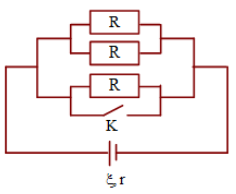
\includegraphics{../figs/VN11-2021-PH-TP016-1.png}
		\end{center}
	Các điện trở có giá trị bằng nhau $R=\SI{6}{\Omega}$. Nguồn điện có suất điện động $\calE=\SI{3}{V}$, điện trở trong $r=\SI{2}{\Omega}$. Điện trở của các dây nối và khóa K không đáng kể. Cường độ dòng điện chạy qua nguồn khi đóng khóa K có giá trị bằng
		\begin{mcq}(4)
			\item $\SI{1.5}{A}$.
			\item $\SI{0.75}{A}$.
			\item $\SI{0.15}{A}$.
			\item $\SI{0.6}{A}$.
		\end{mcq}
		
	}
	\loigiai
	{	\textbf{Đáp án: A.}
		
		Khi đóng khóa K thì mạch bị nối tắt, nên điện trở mạch ngoài bằng không.
		
		Cường độ dòng điện qua mạch:
		$$I=\dfrac{\calE}{r} = \SI{1.5}{A}.$$
	}
	\item \mkstar{2}
	
	\cauhoi
	{Cho mạch điện như hình vẽ.
		\begin{center}
			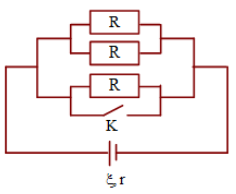
\includegraphics{../figs/VN11-2021-PH-TP016-1.png}
		\end{center}
		Các điện trở có giá trị bằng nhau $R=\SI{6}{\Omega}$. Nguồn điện có suất điện động $\calE=\SI{3}{V}$, điện trở trong $r=\SI{2}{\Omega}$. Điện trở của các dây nối và khóa K không đáng kể. Cường độ dòng điện chạy qua nguồn khi mở khóa K có giá trị bằng
	\begin{mcq}(4)
		\item $\SI{1.5}{A}$.
		\item $\SI{0.75}{A}$.
		\item $\SI{0.15}{A}$.
		\item $\SI{0.6}{A}$.
	\end{mcq}
		
	}
	\loigiai
	{	\textbf{Đáp án: B.}
		
		Khi mở khóa K thì khi đó đoạn mạch gồm ($R$ song song $R$) song song $R$, tương đương với 3 điện trở $R$ mắc song song.
		
		Điện trở tương đương:
		$$R_\text{tđ} = \dfrac{R}{3} = \SI{2}{\Omega}.$$
		
		Cường độ dòng điện qua mạch:
		$$I=\dfrac{\calE}{R_\text{tđ} + r} = \SI{0.75}{A}.$$
	}
	\item \mkstar{2}
	
	\cauhoi
	{Cho mạch điện như hình dưới.
		\begin{center}
			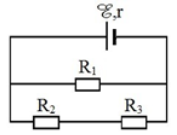
\includegraphics{../figs/VN11-2021-PH-TP016-2.png}
		\end{center}
	Biết $\calE = \SI{12}{V}$, $r=\SI{1}{\Omega}$, $R_1=\SI{5}{\Omega}$, $R_2=R_3=\SI{10}{\Omega}$. Bỏ qua điện trở của dây nối. Hiệu điện thế giữa hai đầu $R_1$ là
		\begin{mcq}(4)
			\item $\SI{10.2}{V}$.
			\item $\SI{4.8}{V}$.
			\item $\SI{9.6}{V}$.
			\item $\SI{7.6}{V}$.
		\end{mcq}
		
	}
	\loigiai
	{	\textbf{Đáp án: C.}
		
		Hiệu điện thế giữa hai đầu $R_1$ cũng là hiệu điện thế mạch ngoài.
		
		Điện trở tương đương mạch ngoài:
		$$R=\dfrac{R_{23} R_1}{R_{23} + R_1} = \SI{4}{\Omega}.$$
		
		Cường độ dòng điện toàn mạch:
		$$I=\dfrac{\calE}{R + r} = \SI{2.4}{A}.$$
		
		Hiệu điện thế mạch ngoài:
		$$U=IR = \SI{9.6}{V}.$$
		
		Vậy $U_1 = U = \SI{9.6}{V}$.
	}
	\item \mkstar{2}
	
	\cauhoi
	{Cho mạch điện như hình dưới.
		\begin{center}
			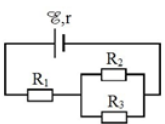
\includegraphics{../figs/VN11-2021-PH-TP016-3.png}
		\end{center}
	Biết $\calE = \SI{9}{V}$, $r=\SI{1}{\Omega}$, $R_1=\SI{5}{\Omega}$, $R_2=\SI{20}{\Omega}$, $R_3=\SI{30}{\Omega}$. Bỏ qua điện trở của dây nối. Hiệu điện thế giữa hai đầu $R_1$ là
		\begin{mcq}(4)
			\item $\SI{8.5}{V}$.
			\item $\SI{6.0}{V}$.
			\item $\SI{4.5}{V}$.
			\item $\SI{2.5}{V}$.
		\end{mcq}
		
	}
	\loigiai
	{	\textbf{Đáp án: D.}
		
		Điện trở tương đương mạch ngoài:
		$$R=R_1 + R_{23} = \SI{17}{\Omega}.$$
		
		Cường độ dòng điện qua mạch:
		$$I=\dfrac{\calE}{R + r} = \SI{0.5}{A}.$$
		
		Hiệu điện thế giữa hai đầu $R_1$:
		$$U_1 = I R_1 = \SI{2.5}{V}.$$
	}
	\item \mkstar{3}
	
	\cauhoi
	{Cho mạch điện như hình vẽ.
		\begin{center}
			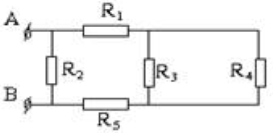
\includegraphics{../figs/VN11-2021-PH-TP016-4.png}
		\end{center}
	
	Trong đó: $R_1=R_3=R_5=\SI{3}{\Omega}$, $R_2=\SI{8}{\Omega}$, $R_4=\SI{6}{\Omega}$, $U_5 = \SI{6}{V}$. Tính điện trở tương đương của đoạn mạch AB và cường độ dòng điện chạy qua từng điện trở.
		\begin{mcq}
			\item $R=\SI{4}{\Omega}$, $I_1=I_5=\SI{2}{A}$, $I_3=\xsi{4/3}{A}$, $I_4=\xsi{2/3}{A}$, $I_2=\SI{2}{A}$.
			\item $R=\SI{8}{\Omega}$, $I_1=I_5=\SI{2}{A}$, $I_3=\xsi{4/3}{A}$, $I_4=\xsi{2/3}{A}$, $I_2=\SI{2}{A}$.
			\item $R=\SI{4}{\Omega}$, $I_1=I_5=\SI{1}{A}$, $I_3=\xsi{4/3}{A}$, $I_4=\xsi{2/3}{A}$, $I_2=\SI{2}{A}$.
			\item $R=\SI{8}{\Omega}$, $I_1=I_5=\SI{2}{A}$, $I_3=\xsi{2/3}{A}$, $I_4=\xsi{4/3}{A}$, $I_2=\SI{2}{A}$.
		\end{mcq}
		
	}
	\loigiai
	{	\textbf{Đáp án: A.}
		
		Điện trở thành phần:
		$$R_{34} = \dfrac{R_3 R_4}{R_3 + R_4} = \SI{2}{\Omega}.$$
		
		$$R_{1345} = R_1 + R_{34} + R_5 = \SI{8}{\Omega}.$$
		
		$$R=\dfrac{R_2 R_{1345}}{R_2 + R_{1345}} = \SI{4}{\Omega}.$$
		
		Cường độ dòng điện:
		$$I_5 = I_{34} = I_1 = I_{1345} = \dfrac{U_5}{R_5} = \SI{2}{A}.$$
		
		Hiệu điện thế:
		$$U_{34} = U_3 = U_4 = I_{34} R_{34} = \SI{4}{V}.$$
		
		Suy ra:
		$$I_3 = \dfrac{U_3}{R_3} = \xsi{\dfrac{4}{3}}{A};\ I_4 = \dfrac{U_4}{R_4} = \xsi{\dfrac{2}{3}}{A};\ U_{1345} = U_2 = U_\text{AB} = I_{1345} R_{1345} = \SI{16}{V};\ I_2 = \dfrac{U_2}{R_2} = \SI{2}{A}.$$
	}
	\item \mkstar{3}
	
	\cauhoi
	{Cho mạch điện như hình vẽ.
		\begin{center}
			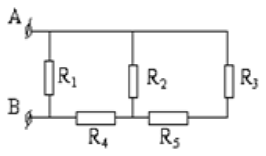
\includegraphics{../figs/VN11-2021-PH-TP016-5.png}
		\end{center}
	Trong đó: $R_1 = \SI{8}{\Omega}$, $R_3=\SI{10}{\Omega}$, $R_2=R_4=R_5=\SI{20}{\Omega}$, $I_3=\SI{2}{A}$. Tính điện trở tương đương của đoạn mạch AB và cường độ dòng điện chạy qua từng điện trở.
		\begin{mcq}
			\item $R=\SI{6.4}{\Omega}$, $I_1=\SI{20}{A}$, $I_2=\SI{3}{A}$, $I_3=I_5=\SI{2}{A}$, $I_4=\SI{5}{A}$.
			\item $R=\SI{32}{\Omega}$, $I_1=\SI{20}{A}$, $I_2=\SI{3}{A}$, $I_3=I_5=\SI{2}{A}$, $I_4=\SI{5}{A}$.
			\item $R=\SI{32}{\Omega}$, $I_1=\SI{4}{A}$, $I_2=\SI{3}{A}$, $I_3=I_5=\SI{2}{A}$, $I_4=\SI{5}{A}$.
			\item $R=\SI{6.4}{\Omega}$, $I_1=\SI{4}{A}$, $I_2=\SI{3}{A}$, $I_3=I_5=\SI{2}{A}$, $I_4=\SI{5}{A}$.
		\end{mcq}
		
	}
	\loigiai
	{	\textbf{Đáp án: A.}
		
		Điện trở thành phần:
		$$R_{35} = R_3 + R_5 = \SI{30}{\Omega}.$$
		
		$$R_{235} = \dfrac{R_2 R_{35}}{R_2 + R_{35}} = \SI{12}{\Omega}.$$
		
		$$R_{4235} = R_4 + R_{235} = \SI{32}{\Omega}.$$
		
		$$R=\dfrac{R_1 R_{4235}}{R_1 + R_{4235}} = \SI{6.4}{\Omega}.$$
		
		Cường độ dòng điện:
		$$I_3 = I_5 = I_{35} = \SI{2}{A}.$$
		
		Hiệu điện thế:
		$$U_{35} = U_2 = U_{235} = I_{35} R_{35} = \SI{60}{V}.$$
		
		Suy ra:
		$$I_2 = \dfrac{U_2}{R_2} = \SI{3}{A};\ I_{235} = I_4 = I_{4235} = \SI{5}{A};\ U_{4235} = U_1 = U_\text{AB} = I_{4235} R_{4235} = \SI{160}{V};\ I_1 = \dfrac{U_1}{R_1} = \SI{20}{A}.$$
	}
	\item \mkstar{3}
	
	\cauhoi
	{Cho mạch điện như hình vẽ.
		\begin{center}
			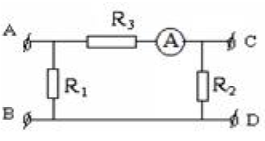
\includegraphics{../figs/VN11-2021-PH-TP016-6.png}
		\end{center}
	Nếu đặt vào AB một hiệu điện thế 100 V thì người ta lấy ra ở hai đầu CD một hiệu điện thế 40 V và ampe kế chỉ 1 A. Nếu đặt vào CD một hiệu điện thế 60 V thì người ta lấy ra ở AB một hiệu điện thế 15 V. Coi điện trở của ampe kế không đáng kể. Tính giá trị của mỗi điện trở.
		\begin{mcq}(2)
			\item $R_1=\SI{30}{\Omega}$, $R_2=\SI{40}{\Omega}$, $R_3=\SI{50}{\Omega}$.
			\item $R_1=\SI{20}{\Omega}$, $R_2=\SI{40}{\Omega}$, $R_3=\SI{60}{\Omega}$.
			\item $R_1=\SI{20}{\Omega}$, $R_2=\SI{30}{\Omega}$, $R_3=\SI{40}{\Omega}$.
			\item $R_1=\SI{30}{\Omega}$, $R_2=\SI{40}{\Omega}$, $R_3=\SI{60}{\Omega}$.
		\end{mcq}
		
	}
	\loigiai
	{	\textbf{Đáp án: B.}
		
		Trường hợp đặt vào giữa A và B hiệu điện thế $\SI{100}{V}$ thì đoạn mạch có: ($R_3$ nối tiếp $R_2$) song song $R_1$, nên:
		$$I_3 = I_2 = I_\text{A} = \SI{1}{A}.$$
		
		$$R_2 = \dfrac{U_\text{CD}}{I_2} = \SI{40}{\Omega}.$$
		
		$$U_\text{AC} = U_\text{AB} - U_\text{CD} = \SI{60}{V}.$$
		
		$$R_3 = \dfrac{U_\text{AC}}{I_3} = \SI{60}{\Omega}.$$
		
		Trường hợp đặt vào giữa C và D hiệu điện thế $\SI{60}{V}$ thì đoạn mạch có: ($R_3$ nối tiếp $R_1$) song song $R_2$. Khi đó:
		$$U_\text{AC} = U_\text{CD} - U_\text{AB} = \SI{45}{V}.$$
		
		$$I_3 = I_1 = \dfrac{U_\text{AC}}{R_3} = \SI{0.75}{A}.$$
		
		$$R_1 = \dfrac{U_\text{AB}}{I_1} = \SI{20}{\Omega}.$$
	}
	\item \mkstar{3}
	
	\cauhoi
	{Cho mạch điện như hình vẽ.
		\begin{center}
			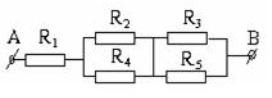
\includegraphics{../figs/VN11-2021-PH-TP016-7.png}
		\end{center}
	Trong đó: $R_1=\SI{2.4}{\Omega}$, $R_3=\SI{4}{\Omega}$, $R_2=\SI{14}{\Omega}$, $R_4=R_5=\SI{6}{\Omega}$, $I_3=\SI{2}{A}$. Tính điện trở tương đương của đoạn mạch AB và hiệu điện thế giữa hai đầu các điện trở.
			\begin{mcq}
			\item $R=\SI{12}{\Omega}$, $U_2 = U_4 = \SI{8}{V}$, $U_1=\SI{8}{V}$, $U_3=U_5=\SI{14}{V}$.
			\item $R=\SI{12}{\Omega}$, $U_2 = U_4 = \SI{14}{V}$, $U_1=\SI{6}{V}$, $U_3=U_5=\SI{8}{V}$.
			\item $R=\SI{12}{\Omega}$, $U_2 = U_4 = \SI{14}{V}$, $U_1=\SI{4}{V}$, $U_3=U_5=\SI{8}{V}$.
			\item $R=\SI{9}{\Omega}$, $U_2 = U_4 = \SI{14}{V}$, $U_1=\SI{8}{V}$, $U_3=U_5=\SI{8}{V}$.
		\end{mcq}
		
	}
	\loigiai
	{	\textbf{Đáp án: D.}
		
		Đoạn mạch gồm: $R_1$ nối tiếp ($R_2$ song song $R_4$) nối tiếp ($R_3$ song song $R_5$).
		
		Điện trở thành phần:
		$$R_{24} = \dfrac{R_2 R_4}{R_2 + R_4} = \SI{4.2}{\Omega}.$$
		
		$$R_{35} = \dfrac{R_3 R_5}{R_3 + R_5} = \SI{2.4}{\Omega}.$$
		
		$$R=R_1 + R_{24} + R_{35} = \SI{9}{\Omega}.$$
		
		Hiệu điện thế:
		$$U_3 = U_5 = U_{35} = I_3 R_3 = \SI{8}{V}.$$
		
		Suy ra:
		$$I_{35} = I_{24} = I_1 = I = \dfrac{U_{35}}{R_{35}} = \xsi{\dfrac{10}{3}}{A};\ U_{24} = U_2 = U_4 = I_{24} R_{24} = \SI{14}{V};\ U_1 = I_1 R_1 = \SI{8}{V}.$$
	}
	\item \mkstar{4}
	
	\cauhoi
	{Cho mạch điện như hình vẽ.
		\begin{center}
			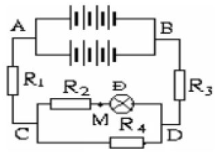
\includegraphics{../figs/VN11-2021-PH-TP016-8.png}
		\end{center}
	Trong đó: bộ nguồn gồm 8 ắcquy, mỗi ắcquy có suất điện động $\calE=\SI{2}{V}$, điện trở trong $r=\SI{0.4}{\Omega}$ mắc thành hai nhánh, mỗi nhánh có 4 nguồn mắc nối tiếp; đèn loại 6 V - 6 W; $R_1=\SI{0.2}{\Omega}$, $R_2=\SI{6}{\Omega}$, $R_3=\SI{4}{\Omega}$ và $R_4=\SI{4}{\Omega}$. Chọn phương án đúng.
		\begin{mcq}(2)
			\item $U_\text{AM} = \SI{-3.4}{V}$ và đèn sáng mạnh.
			\item $U_\text{AM} = \SI{3.4}{V}$ và đèn sáng yếu.
			\item $U_\text{AM} = \SI{-1.7}{V}$ và đèn sáng mạnh.
			\item $U_\text{AM} = \SI{1.7}{V}$ và đèn sáng yếu.
		\end{mcq}
		
	}
	\loigiai
	{	\textbf{Đáp án: D.}
		
		Ta có:
		$$\calP_\text{đ} = I_\text{đ}^2 R_\text{đ} = \dfrac{U_\text{đ}^2}{R_\text{đ}} \Rightarrow R_\text{đ} = \dfrac{U_\text{đ}^2}{\calP_\text{đ}} = \SI{6}{\Omega}.$$
		
		Mạch gồm: $R_1$ nối tiếp [$R_4$ song song ($R_2$ nối tiếp $R_\text{đ}$)] nối tiếp $R_3$.
		$$R_\text{2đ} = R_2 + R_\text{đ} = \SI{12}{\Omega}$$
		
		$$R_\text{2đ4} = \dfrac{R_\text{2đ} R_4}{R_{\text{2đ} + R_4}} = \SI{3}{\Omega}.$$
		
		$$R=R_1 + R_\text{2đ4} + R_3 = \SI{7.2}{\Omega}.$$
		
		Mà:
		$$\calE_\text{b} = 4 \calE = \SI{8}{V};\ r_\text{b} = \dfrac{4r}{2} = \SI{0.8}{\Omega}.$$
		
		$$\Rightarrow I = \dfrac{\calE_\text{b}}{R+r_\text{b}} = \SI{1}{A}.$$
		
		Ta tính được:
		$$U_\text{AC} = I R_1 = \SI{0.2}{V}.$$
		
		$$U_\text{CM} = I_\text{2đ} R_2 = \dfrac{U_\text{2đ}}{R_\text{2đ}} R_2 = \dfrac{U_\text{2đ4}}{R_\text{2đ}} R_2 = \dfrac{I R_\text{2đ4}}{R_\text{2đ}} R_2 = \SI{1.5}{V}.$$
		
		Suy ra:
		$$U_\text{AM} = U_\text{AC} + U_\text{CM} = \SI{1.7}{V}.$$
	}
\end{enumerate}

\whiteBGstarEnd

\loigiai
{
	\begin{center}
		\textbf{BẢNG ĐÁP ÁN}
	\end{center}
	\begin{center}
		\begin{tabular}{|m{2.8em}|m{2.8em}|m{2.8em}|m{2.8em}|m{2.8em}|m{2.8em}|m{2.8em}|m{2.8em}|m{2.8em}|m{2.8em}|}
			\hline
			1.C  & 2.A  & 3.B  & 4.D  & 5.B  & 6.C  & 7.B  & 8.D  & 9.B  & 10.C  \\
			\hline
			11.D  & 12.A  & 13.B  & 14.C  & 15.D  & 16.A  & 17.A  & 18.B  & 19.D  & 20.D  \\
			\hline
		\end{tabular}
	\end{center}
}
\section{Tự luận}
\begin{enumerate}[label=\bfseries Câu \arabic*:]
	\item \mkstar{1}
	
	\cauhoi{
		Toàn mạch là gì? Phát biểu định luật Ôm cho toàn mạch.
	}
	
	\loigiai{
		
		Toàn mạch là mạch điện gồm nguồn điện có suất điện động $\calE$ và điện trở trong $r$ hoặc gồm các nguồn điện được ghép thành bộ, nối với mạch ngoài gồm các điện trở hoặc các vật dẫn được coi như là điện trở.
		
		Định luật Ôm đối với toàn mạch: Cường độ dòng điện chạy trong mạch kín tỉ lệ thuận với suất điện động của nguồn điện và tỉ lệ nghịch với điện trở toàn phần của mạch đó.
		$$I=\dfrac{\calE}{R_\text{N} + r}.$$
	}
	
	\item \mkstar{2}
	
	\cauhoi{
		Một đoạn mạch gồm điện trở $R_1=\SI{100}{\Omega}$ mắc nối tiếp với điện trở $R_2=\SI{200}{\Omega}$, hiệu điện thế giữa hai đầu đoạn mạch là 12 V. Tính hiệu điện thế giữa hai đầu điện trở $R_1$.
	}
	
	\loigiai{
		
		Điện trở tương đương của mạch ngoài:
		$$R=R_1 + R_2 = \SI{300}{\Omega}.$$
		
		Cường độ dòng điện toàn mạch cũng chính là cường độ dòng điện đi qua $R_1$:
		$$I_1 = I =\dfrac{U}{R} = \SI{0.04}{A}.$$
		
		Hiệu điện thế giữa hai đầu $R_1$:
		$$U_1 = U R_1 = \SI{4}{V}.$$
	}
	\item \mkstar{3}
	
	\cauhoi{
	Cho mạch điện như hình vẽ.
	\begin{center}
		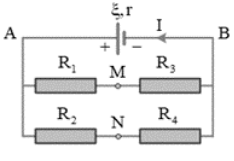
\includegraphics{../figs/VN11-2021-PH-TP016-9.png}
	\end{center}
	Cho $r=\SI{1}{\Omega}$, $R_1=\SI{1}{\Omega}$, $R_2=\SI{4}{\Omega}$, $R_3=\SI{3}{\Omega}$, $R_4=\SI{8}{\Omega}$ và $U_\text{MN} = \SI{1.5}{V}$. Điện trở của các dây nối không đáng kể. Tính suất điện động của nguồn.
	}
	
	\loigiai{
		
		Điện trở tương đương của mạch ngoài:
		$$R=\dfrac{(R_1 + R_3) (R_2 + R_4)}{(R_1 + R_3) + (R_2 + R_4)} = \SI{3}{\Omega}.$$
		
		Hiệu điện thế mạch ngoài:
		$$U_\text{AB} = I R = I_{13} (R_1 + R_3) = I_{24} (R_2 + R_4).$$
		
		Ta được hệ phương trình:
		$$
		\begin{cases}
			I_{13} = I \dfrac{R}{R_1 + R_3} = \SI{0.75}{} I \\
			I_{24} = I \dfrac{R}{R_2 + R_4} = \SI{0.25}{} I.
		\end{cases}
		$$
		
		Xét hiệu điện thế $U_\text{MN}$, ta có:
		$$U_\text{MN} = U_\text{MB} + U_\text{BN} = U_\text{MB} - U_\text{NB} = I_{13} R_3 - I_{24} R_4.$$
		
		Mà $U_\text{MN} = \SI{1.5}{V}$, suy ra:
		$$\SI{1.5}{} = \SI{0.75}{} I \cdot 3 - \SI{0.25}{} I \cdot 8 \Rightarrow I = \SI{6}{A}.$$
		
		Suất điện động của nguồn:
		$$\calE = I (R+r) = \SI{24}{V}.$$
	}
	\item \mkstar{4}
	
	\cauhoi{
		Để xác định điện trở trong của một nguồn điện, một học sinh mắc mạch điện như hình $\text{H}_1$ bên dưới. Đóng khóa K và điều chỉnh con chạy C, kết quả đo được mô tả bởi đồ thị biểu diễn sự phụ thuộc của chỉ số $U$ của vôn kế vào chỉ số $I$ của ampe kế A như hình $\text{H}_2$.
		\begin{center}
			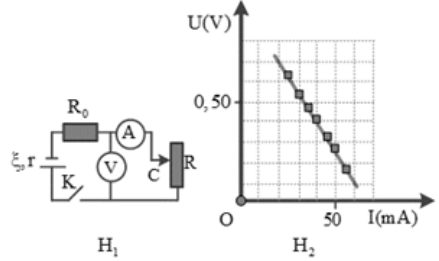
\includegraphics{../figs/VN11-2021-PH-TP016-10.png}
		\end{center}
	Điện trở của vôn kế rất lớn. Biết $R_0=\SI{14}{\Omega}$. Giá trị trung bình của $r$ được xác định bởi thí nghiệm này là bao nhiêu?
	}
	
	\loigiai{
		
		Từ biểu thức:
		$$\dfrac{\calE}{I} = R + R_0 + r.$$
		
		Với $R=\dfrac{U}{I}$, suy ra:
		$$\dfrac{\calE}{I} = \dfrac{U}{I} + R_0 + r.$$
		
		Phương trình trên tương đương với hệ:
		$$
		\begin{cases}
			\dfrac{\calE}{\SI{20e-3}{}} = \dfrac{\SI{0.7}{}}{\SI{20e-3}{}} + 14 + r \\
			\dfrac{\calE}{\SI{60e-3}{}} = \dfrac{\SI{0.1}{}}{\SI{60e-3}{}} + 14 + r
		\end{cases}
		$$
		
		Ta tính được $r=\SI{1}{\Omega}$ và $\calE = \SI{1}{V}$.
		
		Vậy giá trị trung bình của $r$ là $\SI{1}{\Omega}$.
	}
	\item \mkstar{4}
	
	\cauhoi{
		Cho mạch điện như hình vẽ.
		\begin{center}
			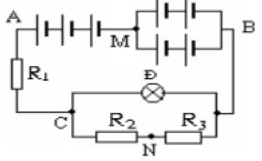
\includegraphics{../figs/VN11-2021-PH-TP016-11.png}
		\end{center}
	Trong đó có 7 nguồn giống nhau, mỗi nguồn có suất điện động $\calE = \SI{2}{V}$, điện trở trong $r=\SI{0.2}{\Omega}$ mắc như hình vẽ. Đèn thuộc loại 6 V - 12 W, cho $R_1=\SI{2.2}{\Omega}$, $R_2=\SI{4}{\Omega}$, $R_3=\SI{2}{\Omega}$. Tính hiệu điện thế $U_\text{MN}$.
	}
	
	\loigiai{
		
		Khi $R_1$ nối tiếp $R_2$ thì cường độ dòng điện qua mỗi điện trở là
		$$I = \dfrac{\calE}{R_1 + R_2 + r} \Rightarrow R_1 + R_2 = \SI{0.9}{\Omega}\ (*).$$
		
		Khi $R_1$ song song $R_2$ thì cường độ dòng điện tổng cộng qua hai điện trở là
		$$I=\dfrac{\calE}{\dfrac{R_1 R_2}{R_1 + R_2} + r} \Rightarrow \dfrac{R_1 R_2}{R_1 + R_2} = \SI{0.2}{\Omega}\ (**).$$
		
		Từ $(*)$ và $(**)$, tính được:
		$$R_1 = \SI{0.6}{\Omega};\ R_2 = \SI{0.3}{\Omega}.$$
	}
	
\end{enumerate}